%General
\documentclass{article}
\usepackage[utf8]{inputenc}
\usepackage{fullpage}

%Symbols
\usepackage{commath}
\usepackage{amsmath}
\usepackage{amssymb}

%Formatting

%%Automata
\usepackage{tikz}
\usetikzlibrary{arrows,automata}

\usepackage{bussproofs}
\usepackage{hyperref}
\usepackage{amsthm}
\usepackage{alltt}
\newtheorem{theorem}{Theorem}[section]
\newtheorem{definition}[theorem]{Definition}
\newtheorem{example}[theorem]{Example}
\hypersetup{colorlinks=true}
\hypersetup{colorlinks=true}
\usepackage{graphicx}
\graphicspath{ {img/} }
\usepackage{caption}

\title{Title}
\date{\today}
\author{Hjort}

\begin{document}
\maketitle

\section*{DFA}
\subsection*{Basic exercises}

\begin{enumerate}
    \item \textbf{Exercise 2.2.4:} Give DFA's accepting the following languages over the alphabet \{0,1\}:

        All these are validated in the Programs folder in this repository, using Erlang

        \begin{enumerate}
            \item The set of all strings ending in $00$.

                $
                \begin{array}{r || c | c}
                        & 0 & 1 \\ \hline \hline
                    \to q_0 & q_1 & q_0 \\
                        q_1 & q_2 & q_0\\
                        *q_2 & q_2 & q_0
                \end{array}
                $

            \item The set of all strings with three consecutive 0's (not necessarliy at the end)

                $ \begin{array}{r||c|c}
                            & 0 & 1 \\ \hline \hline
                    \to q_0 & q_1 & q_0 \\
                    q_1 & q_2 & q_0 \\
                    q_2 & q_3 & q_0 \\
                    *q_3 & q_3 & q_3
                \end{array}
                $

            \item The set of strings with 001 as a substring

                $ \begin{array}{r||c|c}
                            & 0 & 1 \\ \hline \hline
                    \to q_0 & q_1 & q_0 \\
                    q_1 & q_1 & q_2 \\
                    q_2 & q_1 & q_3 \\
                    *q_3 & q_3 & q_3
                \end{array}
                $

        \end{enumerate}

        % 2
    \item
        A language is a regular language iff it is accepted by some finite automata. We thus construct this automata to prove that this is a regular language.

        $ \begin{array}{r||c|c}
            & 0 & 1 \\ \hline \hline
            \to q_0 & q_1 & q_0 \\
            q_1 & q_1 & q_2 \\
            q_2 & q_3 & q_0 \\
            q_3 & q_4 & q_2 \\
            *q_4 & q_1 & q_2
        \end{array}
        $

        \begin{proof}
            (If part) A string ending in 0100 can be in any state when these last digits are encountered. For every state, we follow the arcs labeled 0,1,0,0 in turn and find we always end in $q_4$, which is an accepting state, so the string is accepted.

            (Only if part) A string has been accepted by the DFA. Since it takes a minimum of 4 transitions to get there, the string must be of at least length 4. We can only reach $q_4$ from $q_3$ following a 0, so the last digit must have been 0. We could only get to $q_3$ from $q_2$, following the arc labeled 0, so the string ends in 00. Every arc into $q_2$ is labeled 1, so the string must end in 100. We can get to $q_2$ only from $q_4$, $q_3$ and $q_1$. All these three states only have arcs labeled 0 going int to them, so the string must end in 0100.
        \end{proof}


    \item

        The state diagram for the DFA accpting words containing $bba$ is seen below.

        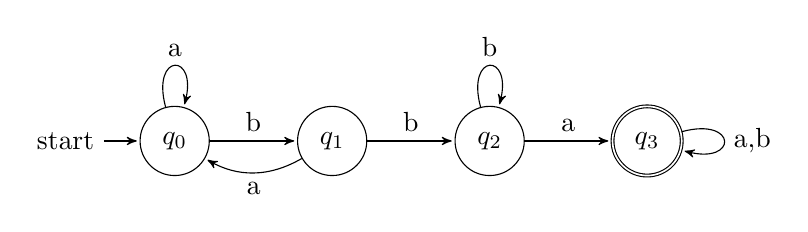
\begin{tikzpicture}[>=stealth',shorten >=1pt,auto,node distance=2cm]
            \node[initial, state]   (q0)    {$q_0$};
            \node[state]            (q1) [right of=q0]    {$q_1$};
            \node[state]            (q2) [right of=q1]    {$q_2$};
            \node[state, accepting] (q3) [right of=q2]    {$q_3$};

            \path[->]
                (q0) edge [loop above]  node {a} (q0)
                     edge   node {b} (q1)
                 (q1) edge  [bend left] node {a} (q0)
                     edge   node {b} (q2)
                (q2) edge   node {a} (q3)
                    edge   [loop above] node {b} (q2)
                (q3) edge  [loop right] node {a,b} (q3);
        \end{tikzpicture}

        The DFA accepting only words without $bba$ as subword must be the words that are not in an accepting state after processing a word with $bba$ as subword, and in an accepting state otherwise. Thus, we simply create an opposite of the DFA above.


        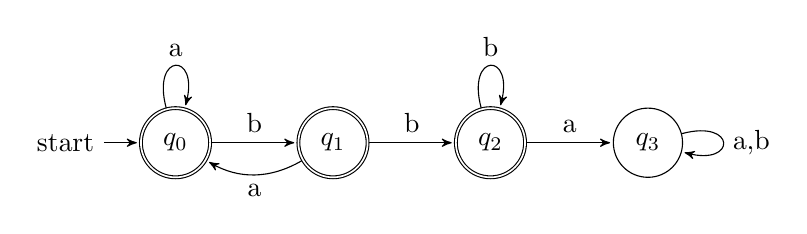
\begin{tikzpicture}[>=stealth',shorten >=1pt,auto,node distance=2cm]
            \node[initial, state, accepting]   (q0)    {$q_0$};
            \node[state, accepting]            (q1) [right of=q0]    {$q_1$};
            \node[state, accepting]            (q2) [right of=q1]    {$q_2$};
            \node[state] (q3) [right of=q2]    {$q_3$};

            \path[->]
                (q0) edge [loop above]  node {a} (q0)
                     edge   node {b} (q1)
                 (q1) edge  [bend left] node {a} (q0)
                     edge   node {b} (q2)
                (q2) edge   node {a} (q3)
                    edge   [loop above] node {b} (q2)
                (q3) edge  [loop right] node {a,b} (q3);
        \end{tikzpicture}

    \item
        \begin{equation*}
            D_1 =
            \begin{array}{r || c | c | c}
                &a  &b  &c \\ \hline \hline
                \to A & B & A & A \\
                B & B & A & C \\
                *C & C & C & C
            \end{array}
        \end{equation*}

        \begin{equation*}
            D_2 =
            \begin{array}{r || c | c | c}
                &a  &b  &c \\ \hline \hline
                \to D & E & D & D \\
                E & E & F & D \\
                *F & F & F & F
            \end{array}
        \end{equation*}

        We then create the DFA $D_3$ which will accept both $ab$ and $ac$ by the product construction.

        \begin{equation*}
        D_3 = (\set{A,B,C} \times \set{D,E,F}, \set{a,b,c}, \delta, AD, \set{C}\times\set{F})
        \end{equation*}

        Where $\delta$ is defined as general in the product rule. We obtain the automata below.

        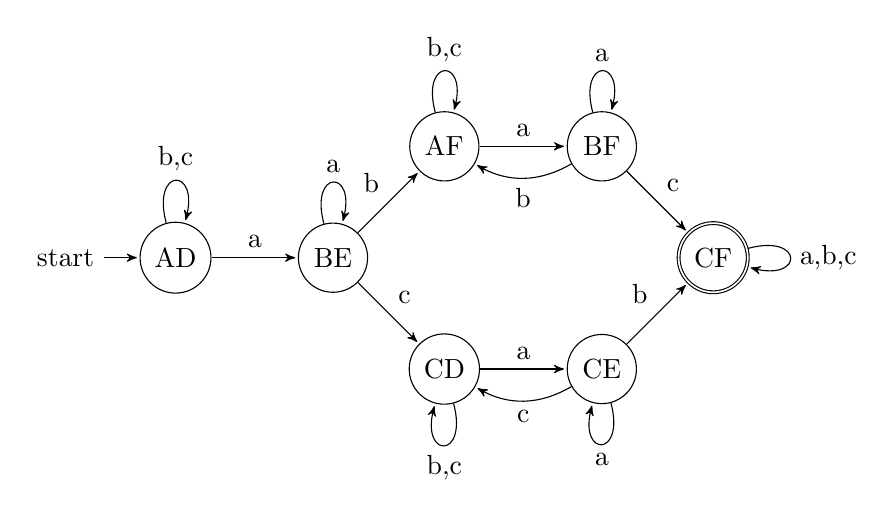
\begin{tikzpicture}[>=stealth',shorten >=1pt,auto,node distance=2cm]
            \node[state, initial] (AD) {AD};
            \node[state] (BE) [right of=AD] {BE};
            \node[state] (AF) [above right of=BE] {AF};
            \node[state] (CD) [below right of=BE] {CD};
            \node[state] (BF) [right of=AF] {BF};
            \node[state] (CE) [right of=CD] {CE};
            \node[state, accepting] (CF) [below right of=BF] {CF};

            \path[->]
                (AD) edge [loop above] node {b,c} (AD)
                    edge node {a} (BE)
                (BE) edge [loop above] node {a} (BE)
                    edge node {b} (AF)
                    edge node {c} (CD)
                (AF) edge [loop above] node {b,c} (AF)
                    edge node {a} (BF)
                (CD) edge [loop below] node {b,c} (CD)
                    edge node {a} (CE)
                (BF) edge [loop above] node {a} (BF)
                    edge [bend left] node {b} (AF)
                    edge node {c} (CF)
                (CE) edge [loop below] node {a} (CE)
                    edge [bend left] node {c} (CD)
                    edge node {b} (CF)
                (CF) edge [loop right] node {a,b,c} (CF)
                   ; 
        \end{tikzpicture}

        For the DFA $D_4$ that accepts $ac$ but not $ab$, we do the product construction of $D_1 \times \overline{D_2}$. The only difference between $D_2$ and its negation is the accepting states, and thus the only difference between $D_3$ and $D_4$ are the accepting states. In $D_4$ the accepting states become $\set{A,B} \times \set{F} = \set{(A,F),(B,F)}$. The automata $D_4$ is shown below.

         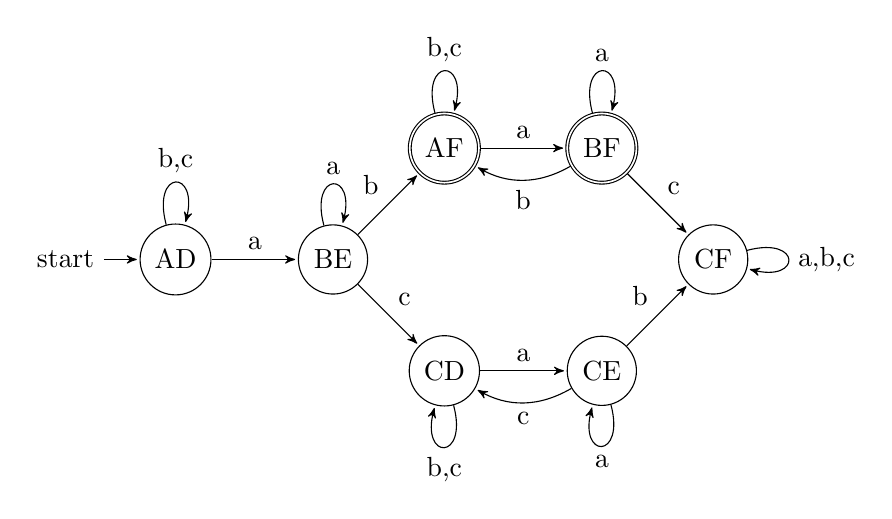
\begin{tikzpicture}[>=stealth',shorten >=1pt,auto,node distance=2cm]
            \node[state, initial] (AD) {AD};
            \node[state] (BE) [right of=AD] {BE};
            \node[state, accepting] (AF) [above right of=BE] {AF};
            \node[state] (CD) [below right of=BE] {CD};
            \node[state,accepting] (BF) [right of=AF] {BF};
            \node[state] (CE) [right of=CD] {CE};
            \node[state] (CF) [below right of=BF] {CF};

            \path[->]
                (AD) edge [loop above] node {b,c} (AD)
                    edge node {a} (BE)
                (BE) edge [loop above] node {a} (BE)
                    edge node {b} (AF)
                    edge node {c} (CD)
                (AF) edge [loop above] node {b,c} (AF)
                    edge node {a} (BF)
                (CD) edge [loop below] node {b,c} (CD)
                    edge node {a} (CE)
                (BF) edge [loop above] node {a} (BF)
                    edge [bend left] node {b} (AF)
                    edge node {c} (CF)
                (CE) edge [loop below] node {a} (CE)
                    edge [bend left] node {c} (CD)
                    edge node {b} (CF)
                (CF) edge [loop right] node {a,b,c} (CF)
                   ; 
        \end{tikzpicture}

    \item
        The language accepted by this DFA is all strings in $\set{0,1}^*$ which have an odd number of 1:s in them.

        Let $w$ be a string in $\set{0,1}^*$. We prove that the above is correct by simple induction on $|w|$.

        We first note that the transition function for this DFA is defined as follows:

        \begin{align*}
            \delta(A,0) = A \\
            \delta(A,1) = B \\
            \delta(B,0) = B \\
            \delta(B,1) = A \\
        \end{align*}

        Let $P(n)$ mean that for strings of length $n$, the only strings accepted are those with an odd number of 1's, and they are all accepted.

        \begin{description}
            \item[Base case]
                $|w|=0 \Rightarrow w = \epsilon$. By definition $\hat{\delta}(q, \epsilon) = q$, so $\hat{\delta}(A,\epsilon) = A$, which is not an accepting state. Since $\epsilon$ contains no 1's, and 0 is an even number, $P(0)$ holds.

            \item[Inductive step]
                Assume $P(n)$. If $|w| = n + 1$ then $w = xa$ where $|x| = n$ and $a \in \set{0,1}$.

                Then $\hat{\delta}(A, w) = \delta(\hat{\delta}(A, x), a)$. Since $P(n)$ holds, we know that $\hat{\delta}(A,x)$ is $A$ if $x$ has an even number of zeroes, ond $B$ if the number is odd.

                We have two cases to consider for $a$: where it is 0, and where it is 1.

                (Case of $a=0$) In this case, we do not transition, but stay in the same state as before. That means $\hat{\delta}(A, w) = \hat{\delta}(A,x)$. Now we also note that $a$ didn't increase the number of 1's, so $w$ contains as many 1's as $x$. Thus, by the inductive hypothesis, we are in A iff $w$ contains an even number of 1's.

                (Case of $a=1$) In this case, we always transition to the other state, and our number of 1's increase by 1. Thus, if $x$ has an even number of 1's, $w$ has an odd number, and vice versa. By the same reasoning as above, if $x$ is accepted then $w$ is not, and vice versa.

                We conclude that $P(n) \Rightarrow P(n+1)$.
                
            \item[Closure]
                Since $P(0) \land (P(n) \Rightarrow P(n+1))$, we conclude $\forall n \in \mathbb{N}. P(n)$.

        \end{description}

\end{enumerate}

\subsection*{Additional exercises}

\begin{enumerate}
    \item 
        We give $D_1$ in two ways:

        $
        \begin{array}{r || c | c | c }
            & a & b & c \\ \hline \hline
            \to *q_0& q_1 & q_0 & q_0 \\
            *q_1 & q_1 & q_2 & q_0 \\
            q_2 & q_2 & q_2 & q_2
        \end{array}
        $

%   \begin{tikzpicture}[>=stealth',shorten >=1pt,auto,node distance=2cm]
        \begin{tikzpicture}[>=stealth',shorten >=1pt,node distance=2cm,auto]
            \node[state,initial,accepting] (q0) {$q_0$};
            \node[state,accepting] (q1) [right of=q0]{$q_1$};
            \node[state] (q2) [below right of=q0] {$q_2$};

            \path[->]
                (q0) edge [loop below] node {b,c} (q0)
                edge [bend left] node {a} (q1)
                (q1) edge [loop right] node {a} (q1)
                    edge node {b} (q2)
                    edge [bend left] node {c} (q0)
                (q2) edge [loop below] node {a,b,c} (q2)
                ;
        \end{tikzpicture}

        And we also give $D_2$ in two ways:

        $
        \begin{array}{r || c | c | c }
            & a & b & c \\ \hline \hline
            \to *p_0& p_0 & p_0 & p_1 \\
            *p_1 & p_0 & p_2 & p_1 \\
            p_2 & p_2 & p_2 & p_2
        \end{array}
        $

        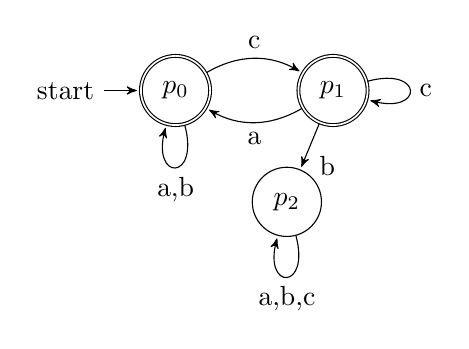
\begin{tikzpicture}[>=stealth',shorten >=1pt,node distance=2cm,auto]
            \node[state,initial,accepting] (p0) {$p_0$};
            \node[state,accepting] (p1) [right of=p0]{$p_1$};
            \node[state] (p2) [below right of=p0] {$p_2$};

            \path[->]
                (p0) edge [loop below] node {a,b} (p0)
                edge [bend left] node {c} (p1)
                (p1) edge [loop right] node {c} (p1)
                     edge node {b} (p2)
                    edge [bend left] node {a} (p0)
                (p2) edge [loop below] node {a,b,c} (p2)
                ;
        \end{tikzpicture}

        One may note that the only difference between these two automata is that all arcs labeled a are now labeled c and vice versa in the diagram, and in the table the columns for a and c has switched places.

        We produce the product of these two automata. We denote that $D_1$ is in state $q_i$ and $D_2$ in state $p_j$ with the combined state $ij$.

        We construct the product automata, $D = \set{Q, \set{a,b,c}, \delta, 00, \set{00,01,10,11}}$ where $Q$ is the set of all states $ij$, $i=0,1,2$  and $j = 0, 1, 2$, and $\delta$ is defined as

        $$\delta((q_i,p_j), s) = (\delta_1(q_i, s), \delta_2(p_j, s))$$

        where $s$ is a symbol on the alphabet and $\delta_1$ and $\delta_2$ are the transition functions of $D_1$ and $D_2$ respectively.

        The result is the following automata:

        $
        \begin{array}{r || c | c | c}
                & a & b & c \\ \hline \hline
            \to *00 & 10 & 00 & 01 \\
            *10 & 10 & 20 & 01 \\
            * 01 & 10 & 02 & 01 \\
            20 & 20 & 20 & 21 \\
            02 & 12 & 02 & 02 \\
            21 & 20 & 22 & 21 \\
            12 & 12 & 22 & 02 \\
            22 & 22 & 22 & 22
        \end{array}
        $

        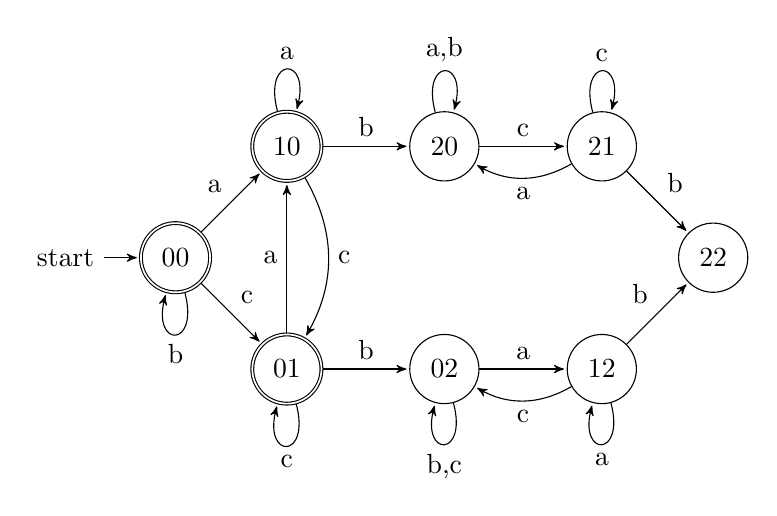
\begin{tikzpicture}[>=stealth', shorten >=1pt, auto, node distance=2cm]
            \node[state, initial, accepting] (00) {00};
            \node[state, accepting] (10) [above right of=00] {10};
            \node[state, accepting] (01) [below right of=00] {01};
            \node[state] (20) [right of=10]{20};
            \node[state] (02) [right of=01]{02};
            \node[state] (21) [right of=20]{21};
            \node[state] (12) [right of=02]{12};
            \node[state] (22) [below right of=21]{22};


            \path[->]
                (00) edge node {a} (10)
                    edge [loop below] node {b} (00)
                    edge  node {c} (01)
                (10) edge [loop above] node {a} (10)
                    edge node {b} (20)
                    edge [bend left] node {c} (01)
                (01) edge node {a} (10)
                    edge node {b} (02)
                    edge [loop below] node {c} (01)
                (20) edge [loop above] node {a,b} (20)
                    edge node {c} (21)
                (02) edge [loop below] node {b,c} (02)
                    edge node {a} (12)
                (21) edge [bend left] node {a} (20)
                    edge node {b} (22)
                    edge [loop above] node {c} (21)
                (12) edge [bend left] node {c} (02)
                    edge node {b} (22)
                    edge [loop below] node {a} (21)
                ;
        \end{tikzpicture}

        We want to prove that this automaton doesn't accept any word where $b$ occurs after $a$ or $c$.

        Let $P(n)$ mean that for all words of length $n$, the automaton rejects words where $b$ occurs after $a$ or $c$.

        \begin{proof}
            Let $w$ be a word. We perform simple induction on $|w|$.

            \begin{description}
                \item[Base case] 
                    After processing the empty string, the automata is in the initial state which is accepting, and $b$ has not occured at all. $\therefore P(0)$.

                \item[Inductive hypothesis]
                    Assume $P(n)$ and let $x$ be a word of length $n$. Let $w = xd$ (we choose the letter $d$ to avoid confusion with our alphabet) so that $|w| = n+1$.

                    Let's first assume that $x$ was rejected by the automaton. Since there are no transitions from a non-accepting state to an accepting state, the automaton must also reject $w$. By our indutive hypothesis, a $b$ occured after an $a$ oor $c$ in $w$, so this is correct.

                    Let's now assume that $x$ was accepted by the automaton. By the inductive hypothesis this means that $x \in b^k\set{a,c}^{n-k}$ for some $0 \leq k \leq n$, meaning that no $b$ has occured after an $a$ or a $c$. Informally, any $b$'s are at the beginning of the word. There are two cases to handle: 
                    \begin{description}
                        \item[First case] There are no $a$'s or $c$'s in the word, so it consists of all $b$'s. Looking at the transition function, we see that $\hat{\delta}(00, b*) = 00$. We also see that for any value of $d$ (recall that $w=xd$) can we transition anywhere other than 00, 10 or 01, which are all accepting. Since the word begins with all $b$'s, $d$ must come after a $b$ and not after any $a$'s or $c$'s, so the automaton should not rjecect, which it doesn't.
                        \item[Second case] There are $a$'s or $c$'s in $x$, meaning, by our inductive hypothesis, that it ends in $a$ or a $c$. We see from the transition function that such a word must be in state 01 or 10, which are both accepting. If $d$ is either $a$ or $c$, then we transition to 01 or 10, which are both accepting. Since no new $b$ has occured, we should accept the string, which we do. However, if $d=b$, then we transition to a non-accepting state. This also means that $x$ contained an $a$ or $c$, which means $w = xb$ has a $b$ after an $a$ or a $c$. We should reject the word, which we do.
                    \end{description}

                    That covers all possible cases: $x$ was rejected, and $x$ was accepted, where the latter had the following sub-cases: $x$ was all b's, $x$ was not all $b$'s. By the law $A \cup \overline{A} = U$, this covers all cases.
                    
                \item[Closure]
                    Since $P(0) \land (P(n) \Rightarrow P(n+1))$ we conclude $\forall n \in \mathbb{N}. P(n)$.
            \end{description}
        \end{proof}
        
\end{enumerate}


